\documentclass[12pt]{article}
\usepackage[utf8]{inputenc}
\usepackage[russian]{babel}
\usepackage{xcolor,colortbl}
\usepackage{graphicx}
\usepackage{subcaption}
\graphicspath{ {./images/} }


\begin{document}

Дубровских Никита 221-361

\textit{\textbf{Вариант 7}}

\textit{\textbf{Задание 17.}}

\textit{Дан взвешенный граф. Найти остов минимального веса
(экстремальное дерево). }

\begin{center}
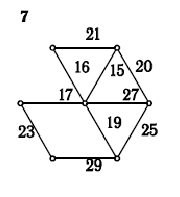
\includegraphics{17.png}
\end{center}

\underline{Решение:}

Найдем ребро минимального веса:

\begin{center}
	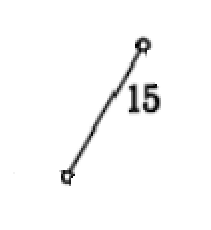
\includegraphics[width=80]{17_1.png}
\end{center}

На
каждом следующем шаге будем брать ребро минимального веса, инцидентное
вершинам, уже включенным в остов и при этом не образующего цикла.

\begin{center}
	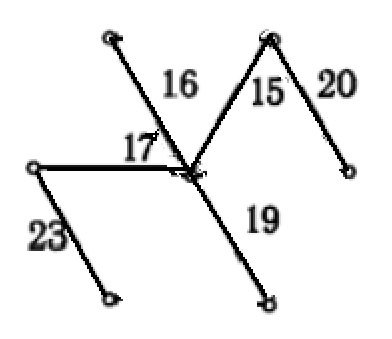
\includegraphics[width=140]{17_2.png}
\end{center}

\textit{\textbf{Задание 18.}}

\textit{Для графа G, заданного матрицей весов, построить минимальный
по весу остов и найти его вес:}

\begin{center}
        \begin{tabular}{ |c|c|c|c|c|c|c|c| }
                \hline
				 & $x_1$ & $x_2$ & $x_3$ & $x_4$ & $x_5$ & $x_6$ & $x_7$\\
                \hline
				x_1 & 0 & 8 & 9 & \infty & \infty & \infty & 6 \\
                \hline
				x_2 & 8 & 0 & 7 & 6 & 9 & \infty & \infty \\
                \hline
				x_3 & 9 & 7 & 0 & 6 & 10 & 5 & \infty \\
                \hline
				x_4 & \infty & 6 & 6 & 0 & 8 & 7 & \infty \\
                \hline
				x_5 & \infty & 9 & 10 & 8 & 0 & 4 & 5\\
                \hline
				x_6 & \infty & \infty & 5 & 7 & 4 & 0 & 6\\
                \hline
				x_7 & 6 & \infty & \infty & \infty & 5 & 6 & 0\\
                \hline
        \end{tabular}
\end{center}

Воспользуемся алгоритмом Краскала. Найдем ребро минимального веса:
$x_5x_6$ - имеет вес 4. На
каждом следующем шаге будем брать ребро минимального веса, инцидентное
вершинам, уже включенным в остов и при этом не образующего цикла.

Покажем последовательно, как добавлялись ребра на матрице графа
(Включенные ячейки закрасим черным, добавляемые – серым). Поскольку граф
не ориентирован, то его матрица симметрична и мы возьмем только ту часть
матрицы, что находится над главной диагональю.

\begin{center}
        \begin{tabular}{ |c|c|c|c|c|c|c|c| }
                \hline
				 & $x_1$ & $x_2$ & $x_3$ & $x_4$ & $x_5$ & $x_6$ & $x_7$\\
                \hline
				x_1 & 0 & 8 & 9 & \infty & \infty & \infty & 6 \\
                \hline
				x_2 & 8 & 0 & 7 & 6 & 9 & \infty & \infty \\
                \hline
				x_3 & 9 & 7 & 0 & 6 & 10 & 5 & \infty \\
                \hline
				x_4 & \infty & 6 & 6 & 0 & 8 & 7 & \infty \\
                \hline
				x_5 & \infty & 9 & 10 & 8 & 0 & \cellcolor{black}\textcolor{white}4 & \cellcolor{gray}5 \\
                \hline
				x_6 & \infty & \infty & 5 & 7 & \cellcolor{black}\textcolor{white}4 & 0 & 6\\
                \hline
				x_7 & 6 & \infty & \infty & \infty & \cellcolor{gray}5 & 6 & 0\\
                \hline
        \end{tabular}
\end{center}

\begin{center}
        \begin{tabular}{ |c|c|c|c|c|c|c|c| }
                \hline
				 & $x_1$ & $x_2$ & $x_3$ & $x_4$ & $x_5$ & $x_6$ & $x_7$\\
                \hline
				x_1 & 0 & 8 & 9 & \infty & \infty & \infty & 6 \\
                \hline
				x_2 & 8 & 0 & 7 & 6 & 9 & \infty & \infty \\
                \hline
				x_3 & 9 & 7 & 0 & 6 & 10 & \cellcolor{gray}5 & \infty \\
                \hline
				x_4 & \infty & 6 & 6 & 0 & 8 & 7 & \infty \\
                \hline
				x_5 & \infty & 9 & 10 & 8 & 0 & \cellcolor{black}\textcolor{white}4 & \cellcolor{black}\textcolor{white}5 \\
                \hline
				x_6 & \infty & \infty & \cellcolor{gray}5 & 7 & \cellcolor{black}\textcolor{white}4 & 0 & 6\\
                \hline
				x_7 & 6 & \infty & \infty & \infty & \cellcolor{black}\textcolor{white}5 & 6 & 0\\
                \hline
        \end{tabular}
\end{center}

\begin{center}
        \begin{tabular}{ |c|c|c|c|c|c|c|c| }
                \hline
				 & $x_1$ & $x_2$ & $x_3$ & $x_4$ & $x_5$ & $x_6$ & $x_7$\\
                \hline
				x_1 & 0 & 8 & 9 & \infty & \infty & \infty & \cellcolor{gray}6 \\
                \hline
				x_2 & 8 & 0 & 7 & 6 & 9 & \infty & \infty \\
                \hline
				x_3 & 9 & 7 & 0 & 6 & 10 & \cellcolor{black}\textcolor{white}5 & \infty \\
                \hline
				x_4 & \infty & 6 & 6 & 0 & 8 & 7 & \infty \\
                \hline
				x_5 & \infty & 9 & 10 & 8 & 0 & \cellcolor{black}\textcolor{white}4 & \cellcolor{black}\textcolor{white}5 \\
                \hline
				x_6 & \infty & \infty & \cellcolor{black}\textcolor{white}5 & 7 & \cellcolor{black}\textcolor{white}4 & 0 & 6\\
                \hline
				x_7 & \cellcolor{gray}6 & \infty & \infty & \infty & \cellcolor{black}\textcolor{white}5 & 6 & 0\\
                \hline
        \end{tabular}
\end{center}

\begin{center}
        \begin{tabular}{ |c|c|c|c|c|c|c|c| }
                \hline
				 & $x_1$ & $x_2$ & $x_3$ & $x_4$ & $x_5$ & $x_6$ & $x_7$\\
                \hline
				x_1 & 0 & 8 & 9 & \infty & \infty & \infty & \cellcolor{black}\textcolor{white}6 \\
                \hline
				x_2 & 8 & 0 & 7 & 6 & 9 & \infty & \infty \\
                \hline
				x_3 & 9 & 7 & 0 & \cellcolor{gray}6 & 10 & \cellcolor{black}\textcolor{white}5 & \infty \\
                \hline
				x_4 & \infty & 6 & \cellcolor{gray}6 & 0 & 8 & 7 & \infty \\
                \hline
				x_5 & \infty & 9 & 10 & 8 & 0 & \cellcolor{black}\textcolor{white}4 & \cellcolor{black}\textcolor{white}5 \\
                \hline
				x_6 & \infty & \infty & \cellcolor{black}\textcolor{white}5 & 7 & \cellcolor{black}\textcolor{white}4 & 0 & 6\\
                \hline
				x_7 & \cellcolor{black}\textcolor{white}6 & \infty & \infty & \infty & \cellcolor{black}\textcolor{white}5 & 6 & 0\\
                \hline
        \end{tabular}
\end{center}

\begin{center}
        \begin{tabular}{ |c|c|c|c|c|c|c|c| }
                \hline
				 & $x_1$ & $x_2$ & $x_3$ & $x_4$ & $x_5$ & $x_6$ & $x_7$\\
                \hline
				x_1 & 0 & 8 & 9 & \infty & \infty & \infty & \cellcolor{black}\textcolor{white}6 \\
                \hline
				x_2 & 8 & 0 & 7 & \cellcolor{gray}6 & 9 & \infty & \infty \\
                \hline
				x_3 & 9 & 7 & 0 & \cellcolor{black}\textcolor{white}6 & 10 & \cellcolor{black}\textcolor{white}5 & \infty \\
                \hline
				x_4 & \infty & \cellcolor{gray}6 & \cellcolor{black}\textcolor{white}6 & 0 & 8 & 7 & \infty \\
                \hline
				x_5 & \infty & 9 & 10 & 8 & 0 & \cellcolor{black}\textcolor{white}4 & \cellcolor{black}\textcolor{white}5 \\
                \hline
				x_6 & \infty & \infty & \cellcolor{black}\textcolor{white}5 & 7 & \cellcolor{black}\textcolor{white}4 & 0 & 6\\
                \hline
				x_7 & \cellcolor{black}\textcolor{white}6 & \infty & \infty & \infty & \cellcolor{black}\textcolor{white}5 & 6 & 0\\
                \hline
        \end{tabular}
\end{center}

Вес: 6+6+5+6+4+5=32

\end{document}
